\documentclass[12pt,a4paper]{article}
\usepackage[utf8]{inputenc}
\usepackage[francais]{babel}
\usepackage[T1]{fontenc}
\usepackage{graphicx}


\usepackage{lipsum}
\usepackage{listings}
\usepackage{enumerate}
\usepackage[backend=bibtex8,backref=true]{biblatex}

\newcommand{\MONTITRE}{Création d'un serveur WEB}
\newcommand{\MONSOUSTITRE}{Installation et configuration}

\addbibresource{dimitri_guedin.bib}
\defbibcheck{online}{\iffieldundef{url}{\skipentry}{}}
\defbibcheck{notonline}{\iffieldundef{url}{}{\skipentry}}

\title{
\begin{tabular}{p{3.5cm} r}
& {\Huge {\bf \MONTITRE}}\\
& {\huge \MONSOUSTITRE}\\
& version du \today{}
\end{tabular}
}


\begin{document}
\maketitle
\newpage
\tableofcontents{}
\newpage

\section{Architecture de la solution}
Le projet consiste à crée un site web qui nous servira de portefeuille de compétences dans le cadre du BTS SIO (Services Informatiques aux Organisations). \\

Le site étant héberger à domicile nous devons donc crée notre propre serveur et en faire la configuration. Nous avons donc choisi de nous tourner vers des solutions libre pour mené a bien ce projet.\\

\textbf{Le serveur web}\newline
Le système d'exploitation qui nous servira de serveur web sera un système GNU/Linux, la distribution Debian. Sur ce serveur nous ajouterons un serveur FTP qui sera par la suite sécurisé.\\

\textbf{Le serveur de base de données}\newline
Nous avons décidé pour des raisons de sécurité de ne pas inclure la base de données du site dans le serveur web, nous allons donc mettre un place un deuxième serveurs ou nous utiliserons une Raspberry Pi pour l'hébergement du serveur de base de données.\\

\textbf{La virtualisation}\newline
Pour des raisons économiques nous avons virtualisée le serveur web, la plateforme de virtualisation que nous avons choisi est nommée Proxmox qui est un système basé sur une distribution Debian.\\

Ce projet englobe donc les deux spécialités de notre BTS, à savoir développement et réseau. La sécurité des serveurs sera une partie importante car nous allons ouvrir le site sur l'extérieur, pour cela nous utiliserons plusieurs outils notamment Nagios pour la supervision des serveurs, failtoban pour la prévention des intrusions et nous sécuriseront nos serveur avec des certificats SSL. 



 
\newpage
\section{Proxmox: Serveur de machines virtuelles}

Proxmox VE est une solution open source complète de virtualisation pour serveurs. Il est basé sur les technologies de virtualisation KVM et conteneurs et gère les machines virtuelles, le stockage, les réseaux virtualisés, et la haute disponibilité.

Les fonctionnalités avancées et l'interface Web intuitive sont conçues pour vous aider à optimiser l'utilisation de vos ressources existantes, réduire les coûts en matériel et le temps nécessaire à l'administration - en entreprise ainsi qu'à la maison. Vous pouvez facilement virtualiser les charges de travail les plus élevées sous Linux et Windows.

\subsection{Installation}

\begin{figure}[!ht]
\center
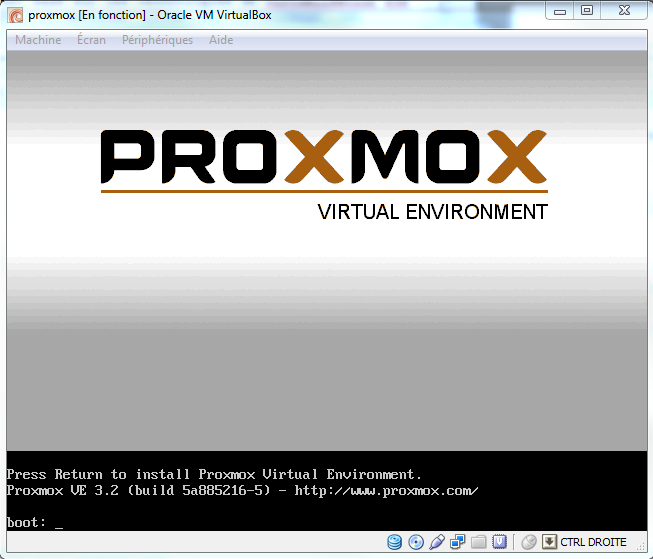
\includegraphics[width=10cm]{Images/1.PNG} 
\caption{Pour continuer appuyer sur "Entrer"}
\end{figure}


\begin{figure}[!ht]
\center
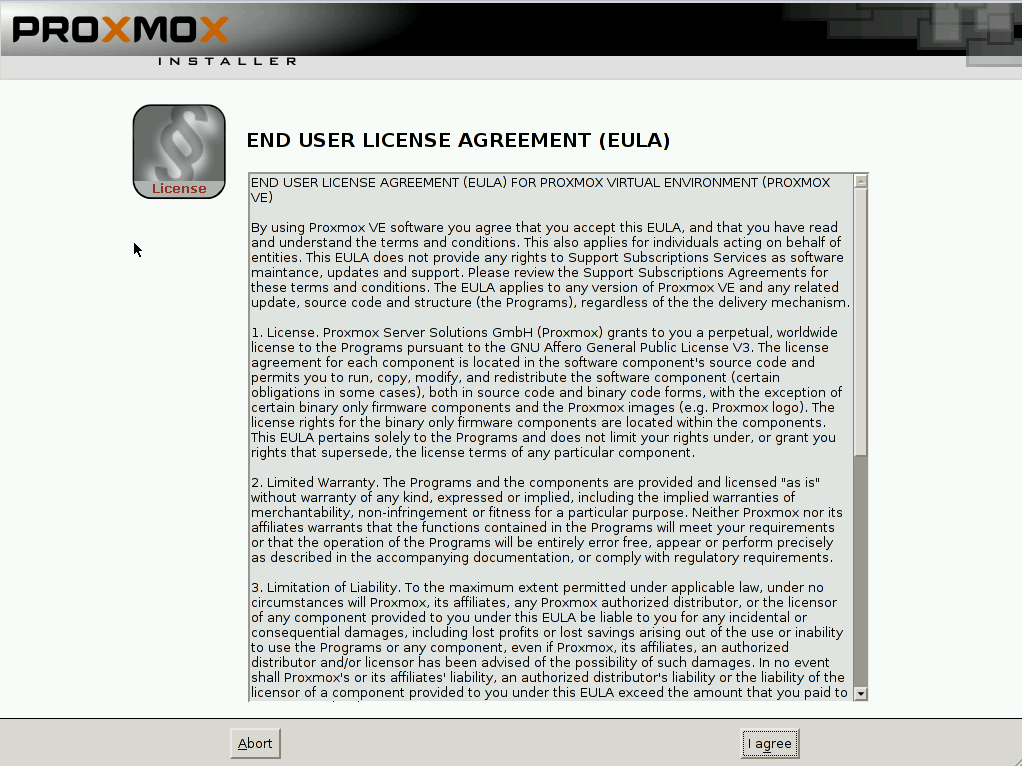
\includegraphics[width=10cm]{Images/2.PNG} 
\caption{Accepter les conditions en cliquant sur "I agree"}
\end{figure}

\begin{figure}[!ht]
\center
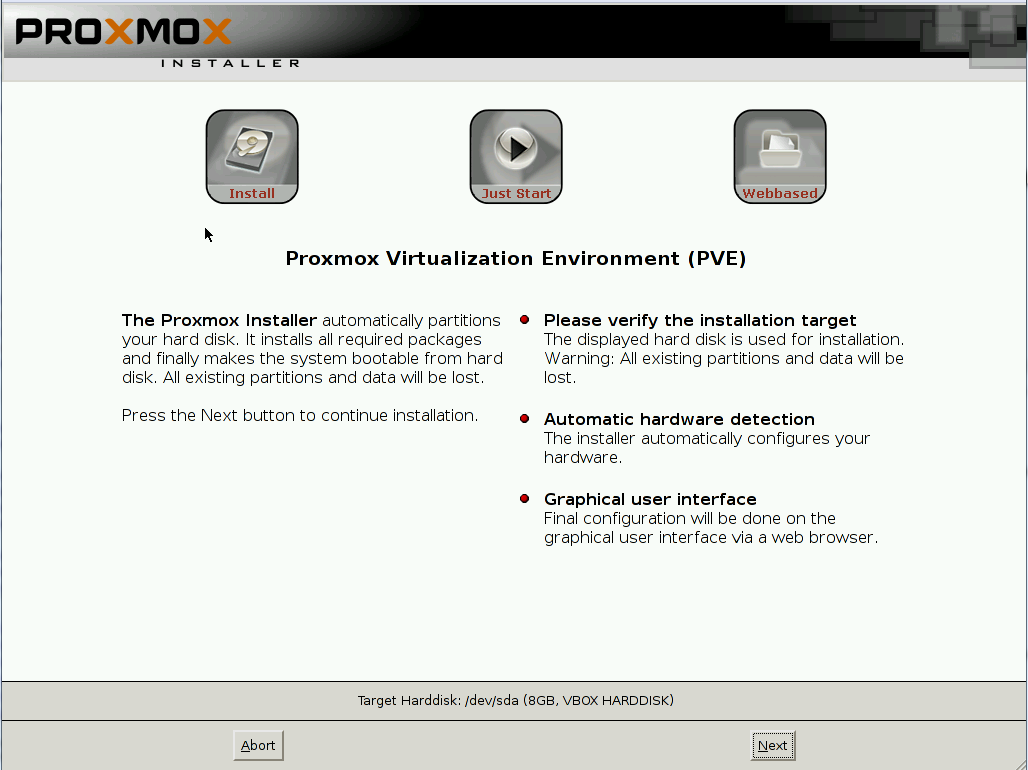
\includegraphics[width=10cm]{Images/3.PNG}  
\caption{Choisir le disque pour l'installation}
\end{figure}


\begin{figure}[!ht]
\center
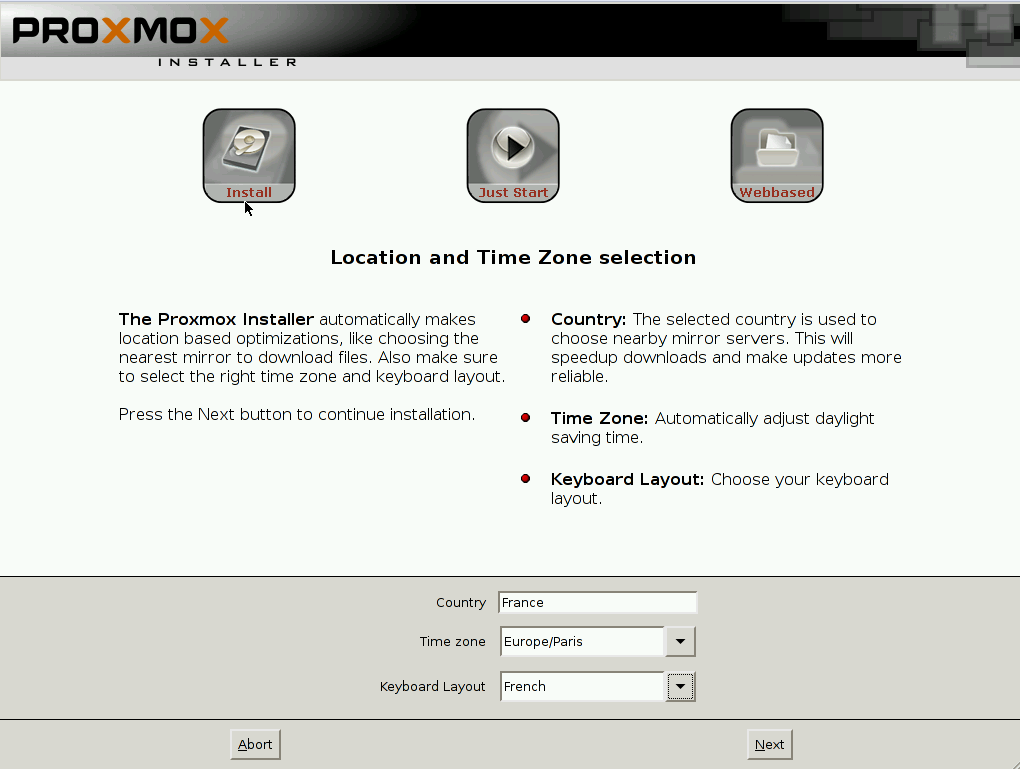
\includegraphics[width=10cm]{Images/4.PNG}  
\caption{Localisation et choix du clavier}
\end{figure}

\begin{figure}[!ht]
\center
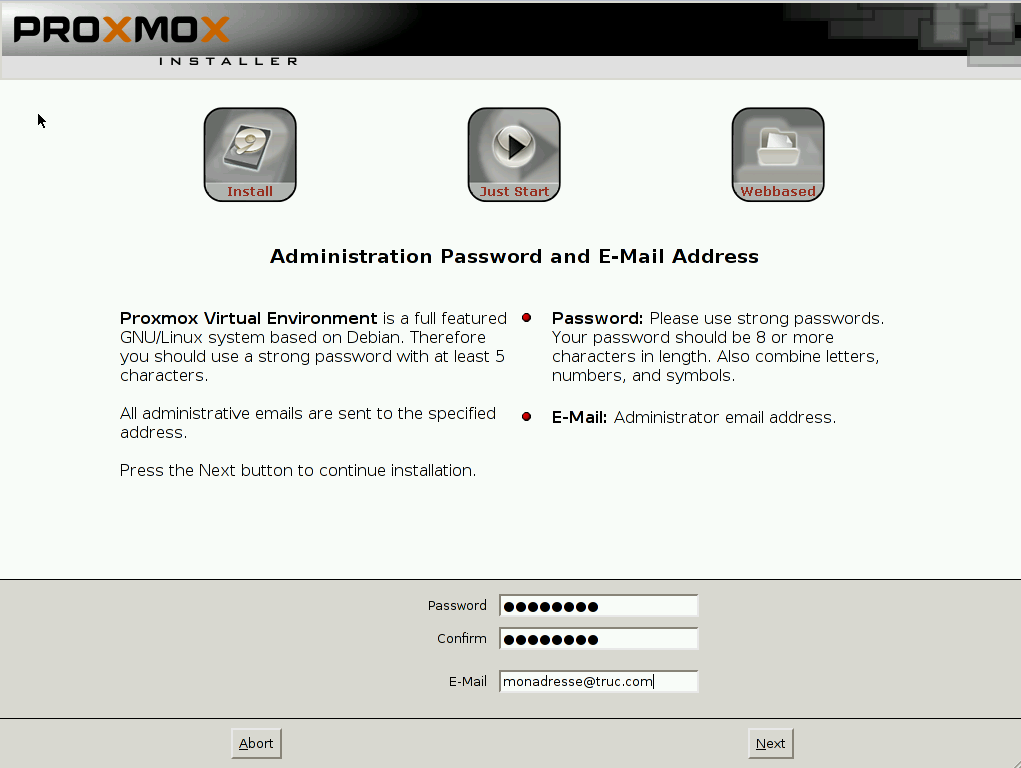
\includegraphics[width=10cm]{Images/5.PNG}  
\caption{Localisation et choix du clavier}
\end{figure}






\end{document}
